\documentclass[10pt,a4paper]{article}
\usepackage{hyperref}
% \usepackage{times,latexsym}
\usepackage[T1]{fontenc}
% \usepackage[]{../common/acl2021}
% \usepackage[]{../common/tacl2018v2}

% replacement for style file
\usepackage{natbib}
% \usepackage{hyperref}
% \usepackage{url}
% \renewcommand{\UrlFont}{\ttfamily\small}

\usepackage{times}
\usepackage{latexsym}

\usepackage{url}
\renewcommand{\UrlFont}{\ttfamily\small}
\usepackage[utf8]{inputenc}
\usepackage{xcolor}

% Totally tabular!
\usepackage{booktabs}

\usepackage{graphicx}

\usepackage{caption}
\usepackage{subcaption}

\usepackage{amssymb}
\usepackage{amsmath}

\usepackage{textcomp}

\DeclareMathOperator*{\argmax}{argmax}
\DeclareMathOperator*{\argmin}{argmin}
\DeclareMathOperator*{\softmax}{softmax}
\DeclareMathOperator*{\logsumexp}{logsumexp}
\DeclareMathOperator*{\hardmax}{hardmax}
\DeclareMathOperator*{\entropy}{H}
\DeclareMathOperator{\expectation}{\mathbb{E}}
\DeclareMathOperator{\prob}{P}

\usepackage{hyperref}
\usepackage{cleveref}
\def\sectionautorefname{Section}
\def\subsectionautorefname{Section}

% (From ACL style:)
% This is not strictly necessary, and may be commented out,
% but it will improve the layout of the manuscript,
% and will typically save some space.
\usepackage{microtype}

% TODO: get a better draft watermark than this lol
% \usepackage{draftwatermark}
% \SetWatermarkText{DRAFT}
% \SetWatermarkScale{1}

% fix up author superscripts
\newcommand*\samethanks[1][\value{footnote}]{\footnotemark[#1]}
\renewcommand*{\Affilfont}{\normalsize\normalfont}
\renewcommand*{\Authfont}{\bfseries}
\renewcommand\footnotemark{}
\makeatletter
\renewcommand\AB@authnote[1]{\rlap{\textsuperscript{\normalfont#1}}}
\renewcommand\Authsep{,~~\,}
\renewcommand\Authand{~~and~}
\renewcommand\Authands{,~~and~}
\makeatother
% end fix up author superscripts

% appendix autoref patch (\autoref subsections in appendix)
% https://tex.stackexchange.com/questions/149807/autoref-subsections-in-appendix
\usepackage{appendix}
\usepackage{etoolbox}
\makeatletter
\patchcmd{\hyper@makecurrent}{%
    \ifx\Hy@param\Hy@chapterstring
        \let\Hy@param\Hy@chapapp
    \fi
}{%
    \iftoggle{inappendix}{%true-branch
        % list the names of all sectioning counters here
        \@checkappendixparam{chapter}%
        \@checkappendixparam{section}%
        \@checkappendixparam{subsection}%
        \@checkappendixparam{subsubsection}%
        \@checkappendixparam{paragraph}%
        \@checkappendixparam{subparagraph}%
    }{}%
}{}{\errmessage{failed to patch}}

\newcommand*{\@checkappendixparam}[1]{%
    \def\@checkappendixparamtmp{#1}%
    \ifx\Hy@param\@checkappendixparamtmp
        \let\Hy@param\Hy@appendixstring
    \fi
}
\makeatletter

\newtoggle{inappendix}
\togglefalse{inappendix}

\apptocmd{\appendix}{\toggletrue{inappendix}}{}{\errmessage{failed to patch}}
\apptocmd{\subappendices}{\toggletrue{inappendix}}{}{\errmessage{failed to patch}}
% end appendix autoref patch

% fancy underline
% https://alexwlchan.net/2017/10/latex-underlines/
\usepackage{contour}
\usepackage[normalem]{ulem}

\renewcommand{\ULdepth}{1.8pt}
\contourlength{0.8pt}

\newcommand{\nuline}[1]{%
  \uline{\phantom{#1}}%
  \llap{\contour{white}{#1}}%
}
% end fancy underline


\usepackage{todonotes}  % temporary - use this for margin notes in bubbles
\usepackage[normalem]{ulem}  % for \sout
\newif\ifcomments
\commentstrue
% \commentsfalse

\ifcomments
    \newcommand*{\TODO}[1]{\textcolor{red}{[TODO: #1]}}
    \newcommand*{\tocite}[1]{(\textcolor{blue}{#1})}
    \newcommand*{\tocitep}[1]{(\textcolor{blue}{#1})}
    \newcommand*{\tocitet}[1]{\textcolor{blue}{#1}}
    
    \newcommand*{\julian}[1]{\textcolor{orange}{[JJM: #1]}}
    \newcommand*{\ian}[1]{\textcolor{olive}{[IFT: #1]}}
    \newcommand*{\jan}[1]{\textcolor{purple}{[JAB: #1]}}
    
    \definecolor{iansnotecolor}{RGB}{255, 218, 181}
    \newcommand*{\iansidenote}[1]{
        \todo[color=iansnotecolor, size=\footnotesize]{%
        [\textbf{Ian:}] #1}%
    }
    
    \newcommand*{\proposed}[1]{\textcolor{purple}{#1}}
    \newcommand*{\maybedelete}[1]{\textcolor{red}{\sout{#1}}}
    \newcommand{\punch}[0]{\includegraphics[width=.04\textwidth]{images/falconpunch.png}}
\else
    %%
    % Disable user commands for submission or length check
    \newcommand*{\TODO}[1]{}
    \newcommand*{\tocite}[1]{}
    \newcommand*{\tocitep}[1]{}
    \newcommand*{\tocitet}[1]{}
    
    \newcommand*{\julian}[1]{}
    \newcommand*{\ian}[1]{}
    \newcommand*{\jan}[1]{}
    \newcommand*{\iansidenote}[1]{}
    
    \newcommand*{\maybedelete}[1]{}
    \newcommand*{\proposed}[1]{#1}
\fi
\usepackage{enumitem}
% \usepackage[margin=1.2in]{geometry}

% \usepackage{csquotes}

% \usepackage{titling}
% \setlength{\droptitle}{-120pt}
% \predate{\vspace{-50pt}\begin{center}\large}
% \postdate{\par\end{center}\vspace{-10pt}}

\newcommand{\ie}{i.e.}
\newcommand{\eg}{e.g.}
\newcommand{\ia}{\textit{inter alia}}


\title{Proposal: An Ambiguous Evaluation of Adversarial Evaluation}

\author{Julian Michael}
\author{Margaret Li}
\affil{CSE 599: Empirical Foundations of Machine Learning \\
Paul G. Allen School of Computer Science \& Engineering, University of Washington \texttt{\{julianjm,margsli\}@cs.washington.edu}}

\date{}

\begin{document}

\maketitle

%%\begin{abstract}
%%  Adversarial evaluation and training have been proposed
%%\end{abstract}

\section*{Introduction}
End-to-end neural network models have had widespread success on standard benchmarks in NLP
\citep{wang2018glue,wang2019superglue,lee2017end,dozat2017deep}.
However, models trained in the standard Empirical Risk Minimization paradigm (\eg, using
maximum-likelihood objectives) are liable to succeed in these settings by fitting to features or
correlations in the data which are ultimately not representative of the underlying task and fail to
generalize out of distribution, \eg, under domain shift or adversarial perturbation
\citep{gururangan2018annotation,ilyas-etal-2019-adversarial}.
One promising method to overcome this difficulty is to move past the ERM paradigm and learn or
evaluate causal features which are invariant across domains or distributions of data.
While methods to do this often require the use of explicitly specified domains of data
% (cite DRO stuff)
\citep{peters-etal-2016-causal,arjovsky-etal-2020-invariant},
a more lightweight approach is adversarial evaluation and training
\citep{nie-etal-2020-adversarial,kiela-etal-2021-dynabench} which has annotators deliberately search
for examples on which a model fails.
Adversarial evaluations can help expose a model's shortcomings
% cite example
and aid in training
more robust models.
However, the process of developing adversarial data is imperfect, and adversarial data may itself
not resemble naturalistic distributions.
For these reasons, it is not clear what a model's performance under adversarial evaluation implies
about its performance characteristics on naturalistic distributions,
and it is not clear in what ways training on adversarial data will aid a model's performance in
natural settings.

In this project, we propose to investigate the interplay of adversarial learning and evaluation with
\textit{ambiguity}, or annotator disagreement.
This is relevant because adversarial data collection can result in strange or unnatural inputs as annotators try tricks to fool a model. To make sure this isn't a problem, such methods often require extra validation of human agreement in order to ensure quality; low-agreement examples are discarded \citep{nie-etal-2020-adversarial}.
%This is relevant because searching for adversarial examples may end up either oversampling
%ambiguous/arguable examples that humans are likely to get `wrong', or, if the data is filtered for
%high human agreement, it may systematically \textit{under}sample such cases.
%In the former case, training on this data may have limited benefits, and in the latter case,
%adversarial evaluation might underestimate model performance in realistic settings.
This potentially introduces a systematic bias in adversarial data which downsamples ambiguous or arguable inputs, which nevertheless may appear frequently in the wild.
The implications of training on such biased data for model behavior on ambiguous or arguable examples are unclear, and may be undesirable (\eg, the model may be overconfident on such examples).
If such shortcomings are present, it would be important for us to understand them.

\paragraph{Research Question}
Do adversarial evaluation or training methods introduce systematic biases that ultimately
misrepresent a model's worst-case performance? In particular, do biases with respect to the
underlying ambiguity of the underlying data limit the benefits of the adversarial approach?

\section*{Experimental Design}

\paragraph{Task Setting}
We will use Natural Language Inference \citep{dagan2005pascal,bowman2015large} as our underlying task, as there exist adversarial annotations for this task \citep{nie-etal-2020-adversarial,kiela-etal-2021-dynabench} and annotator disagreement has been well studied \citep{pavlick-kwiatkowski-2019-inherent,nie-bansal-2020-learn,zhang-de-marneffe-2021-identifying}.

\paragraph{Model Variants}
We will train models under two conditions:
\begin{itemize}
    \item \textbf{Classical:} These models will be trained on data elicited from annotators in a model-agnostic way, \ie, naturalistically.\footnote{Unfortunately, since the NLI task is somewhat artificial, there is no ``natural'' distribution of input texts --- which is one of the issues that leads to annotation artifacts in the first place \citep{gururangan2018annotation} since some of the input text must be annotator-generated. Regardless, spurious correlations exist in any naturalistic distribution so we will use these training sets as proxies for something naturalistic.} For this we use the SNLI \citep{bowman2015large} and MultiNLI \citep{williams-etal-2018-broad} datasets.
    \item \textbf{Adversarial}: These models will be trained on data elicited from annotators under the requirement that they must fool the model. For this we will use the adversarial annotations of \citet{nie-etal-2020-adversarial}.\footnote{In order for this to properly count as adversarial data for our model, we will use the same model family as \citet{nie-etal-2020-adversarial}, which was BERT-large \citep{devlin2019bert} fine-tuned on SNLI and MultiNLI.}
\end{itemize}

\paragraph{Evaluation Data}
The working theory of research on adversarial training and evaluation is that models trained on adversarially-sourced data will be more robust under difficult evaluations, and that models that perform well under adversarial evaluation will be more robust in a variety of settings. We will test those claims in the setting where we have comprehensive distributions of annotator behavior. For this, we will use the ChaosNLI evaluation set \citep{nie-bansal-2020-learn} which has 100 independent annotations for each example (where the task is 3-way multiclass classification).

\paragraph{Metrics}
Using densely-annotated evaluation data, we will compute several evaluation metrics:
\begin{itemize}
    \item \textbf{Expected Accuracy:} The expectation of the accuracy of the model assuming annotators' labels are sampled from their empirical distribution in ChaosNLI.
    \item \textbf{Majority-Vote Accuracy:} The accuracy of the model against the majority vote of the 100 annotators.
    \item \textbf{KL-Divergence:} The KL-divergence of the model's predicted label distribution against the empirical distribution of annotated labels.
    \item \textbf{Model perplexity:} The exponentiated entropy of the model's predicted distribution; higher corresponds to a more uncertain distribution. (This is independent of the gold labels.)
\end{itemize}
For the first two, we can compute their values using a random human from the empirical distribution as a baseline. (For KL-divergence, this value is 0 by construction.)
Expected accuracy emulates the typical accuracy computation in an IID empirical risk minimization setting. Majority-vote accuracy allows us to measure accuracy above human performance. And KL-divergence will show the extent to which the model learns to reproduce the label distribution produced by annotators.

\begin{figure*}[t!]
\centering
\begin{subfigure}[b]{0.48\textwidth}
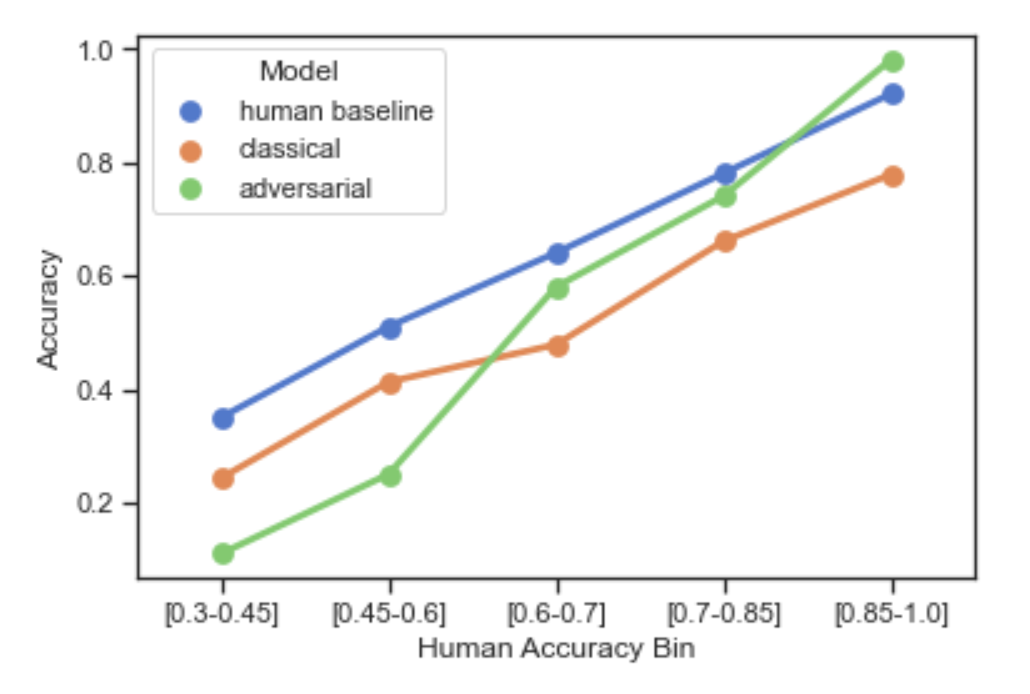
\includegraphics[width=\textwidth]{images/acc.png}
\caption{Expected accuracy stratified by human expected accuracy. In these hypothetical results, the adversarial model performs robustly on high-agreement examples, but degrades on low-agreement examples because these are undersampled in training.\label{fig:accuracy}}

\end{subfigure}
\hfill
\begin{subfigure}[b]{0.48\textwidth}
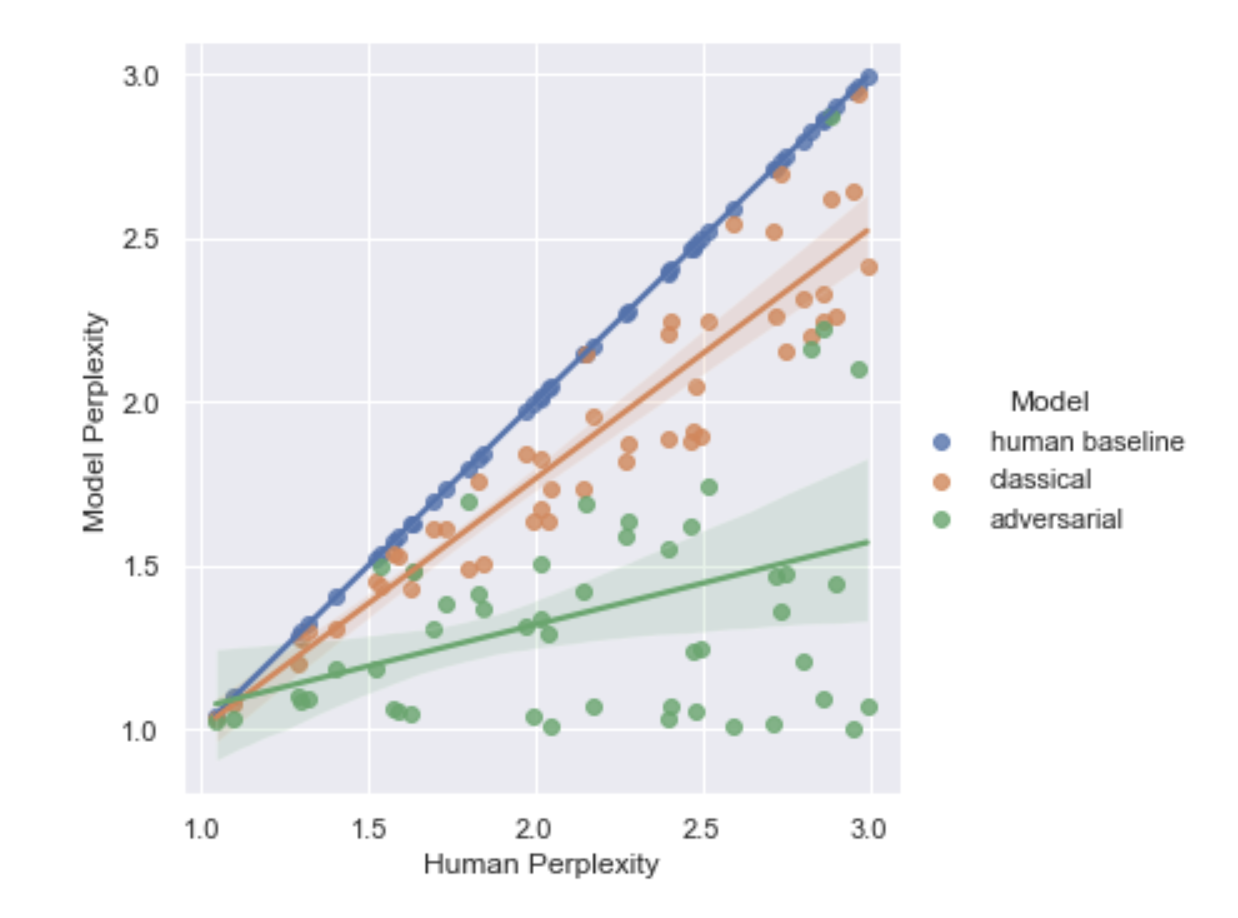
\includegraphics[width=\textwidth]{images/ppl.png}

\caption{Model perplexity, stratified by human perplexity. In these hypothetical results, the adversarially-trained model is disproportionately overconfident on ambiguous examples, since high-agreement examples were overrepresented for it at training time.\label{fig:perplexity}}
\end{subfigure}
\caption{Hypothetical results.\label{fig:mock-graphs}}
\end{figure*}

\paragraph{Analysis}
To more deeply understand our models' performance on ambiguous examples, we will \textbf{stratify our metrics by agreement}. We will stratify examples by two measures of agreement:
\begin{itemize}
    \item \textbf{Human expected accuracy:} low corresponds to low agreement; high is high agreement. On this graph, human performance on expected accuracy would be the $y=x$ diagonal.
    \item \textbf{Human perplexity:} the exponentiated entropy of the distribution of annotator labels. Low corresponds to high agreement; high is low agreement. If the model perfectly matches the human label distribution, its perplexity would equal human perplexity and it would fall on the $y=x$ diagonal. In the case where $y$ is KL-divergence or model perplexity, we can directly use a scatter plot instead of binning.
\end{itemize}
A couple of hypothetical example results graphs for this are shown in \autoref{fig:mock-graphs}.

\section*{Impact}
Example results that we would be looking for are:
\begin{itemize}
    \item A relative lack of performance improvement on ambiguous examples by adversarially-trained models (\autoref{fig:accuracy}). If the performance improvement reliably tracks inversely with example ambiguity, we may be able to estimate the positive effect of adversarial training as a function of the ambiguity rates in new naturalistic data sets. 
    \item Overconfidence on ambiguous examples (\autoref{fig:perplexity}). If adversarial training results in such overconfidence, then mitigation measures may be prudent for the deployment of such models.
\end{itemize}
Adversarial data collection requires extra data filtering; if this introduces systematic biases which cause undesirable model behavior on ambiguous data (such as overconfidence or degraded performance) then mitigations will be important to consider prior to deployment of such models in naturalistic settings.



\bibliographystyle{acl_natbib}
\bibliography{references}
% \bibliography{anthology,references}

\end{document}